\chapter{Logging into Obidos}

The default login screen is shown in the following figure.

\begin{figure}[H]
\centering
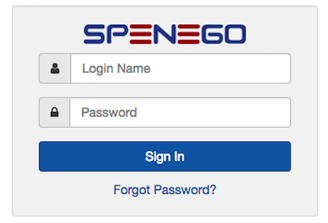
\includegraphics[scale=1.0]{user/Login-Screen.png}
\caption{Obidos Login Screen}
\label{fig: Figure}
\end{figure}

\section{Username and Password}
In order to log into Obidos a user needs a username and password.
If the user account is maintained completely within Obidos, it is a local account.
For local accounts, the username and password are both managed within Obidos.

If the user account is set up for single signon using corporate directory service,
the username and password must be entered as they are in the corporate directory.

\subsection{Local Password}
User passwords issued by Obidos will follow the password policies set in Obidos.
Initially the Administrator will set a temporary password.
The Administrator can choose to send an email to the User informing that an account has been created.
The first time the User logs in using temporary password, Obidos will prompt the User to set
permanent password that conforms to the password policy.

\begin{figure}[H]
\centering
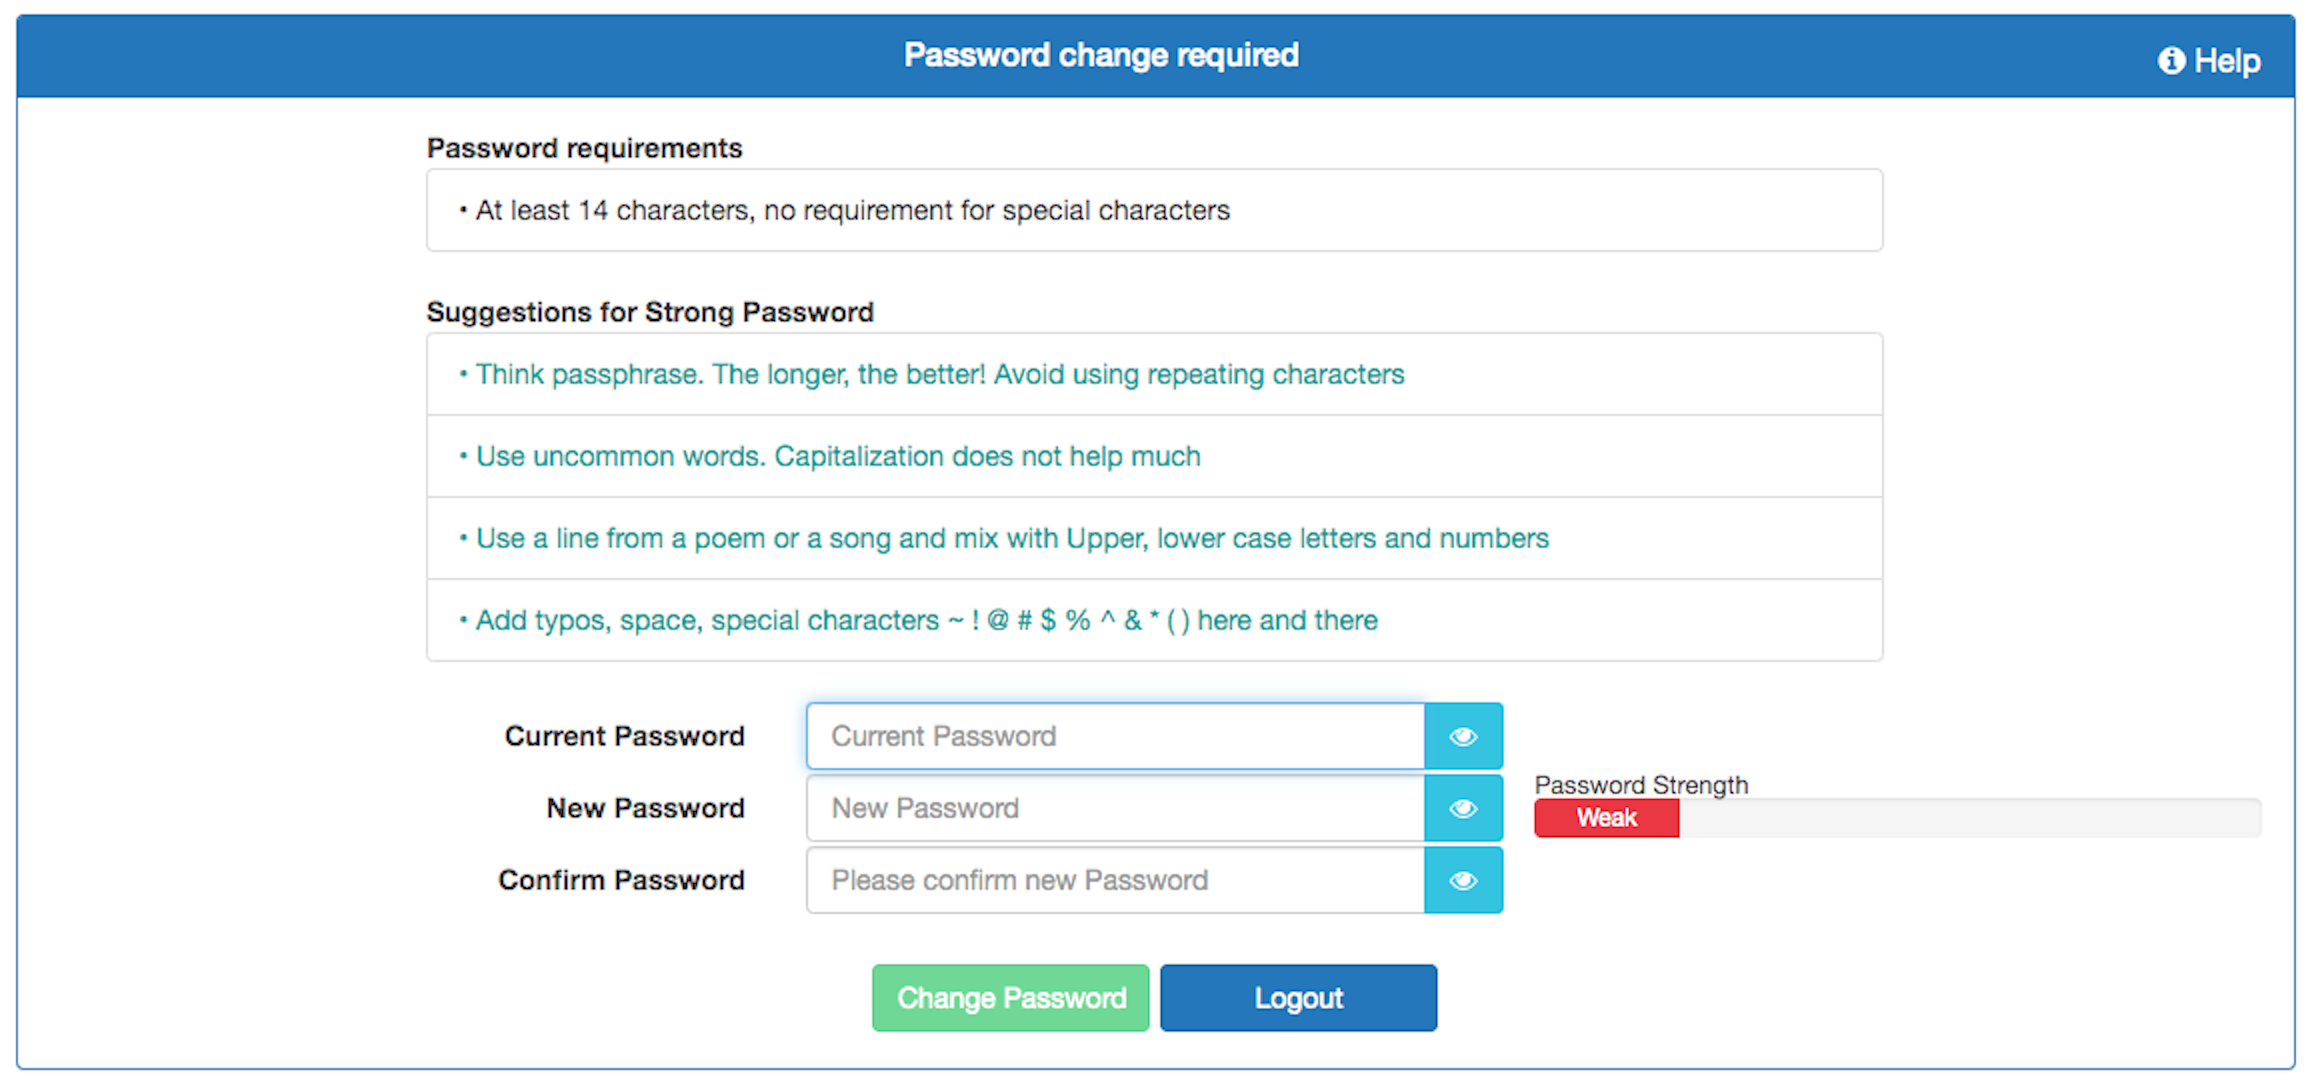
\includegraphics[scale=0.4]{user/Change-Temp-Password.png}
\caption{Change Temporary Password}
\label{fig: Figure}
\end{figure}

Once the new password is set, the User will be logged out of Obidos and prompted to log in using the new password.

\subsection{Directory-synchronized Password}
If a user password is synchronized with the corporate directory service, Obidos will
pass the User credentials to the corporate directory service to be validated.
In this case, Obidos do not have any control on the password.

\section{Passphrase}
When an Item is stored in Obidos, it is encrypted using one key from the personal key pair and
when the Item is retrieved, it is decrypted using the other key.
Such a private key pair is personalized using a passphrase that is chosen by the User.
Passphrase is a string that the User selects.
These passphrases are not stored in Obidos. The user will have to remember the passphrase.
Obidos will generate key pair (private \& public) for each user using the User's passphrase.
In order to retrieve an Item stored in Obidos, the User will need to provide the passphrase.
\textcolor{red}{If the User forgets the passphrase, it is not possible to retrieve any Item stored in the User's Containers.}

When logging into Obidos for the very first time, a user will be prompted to set the passphrase as shown in the following Figure. 

\begin{figure}[H]
\centering
%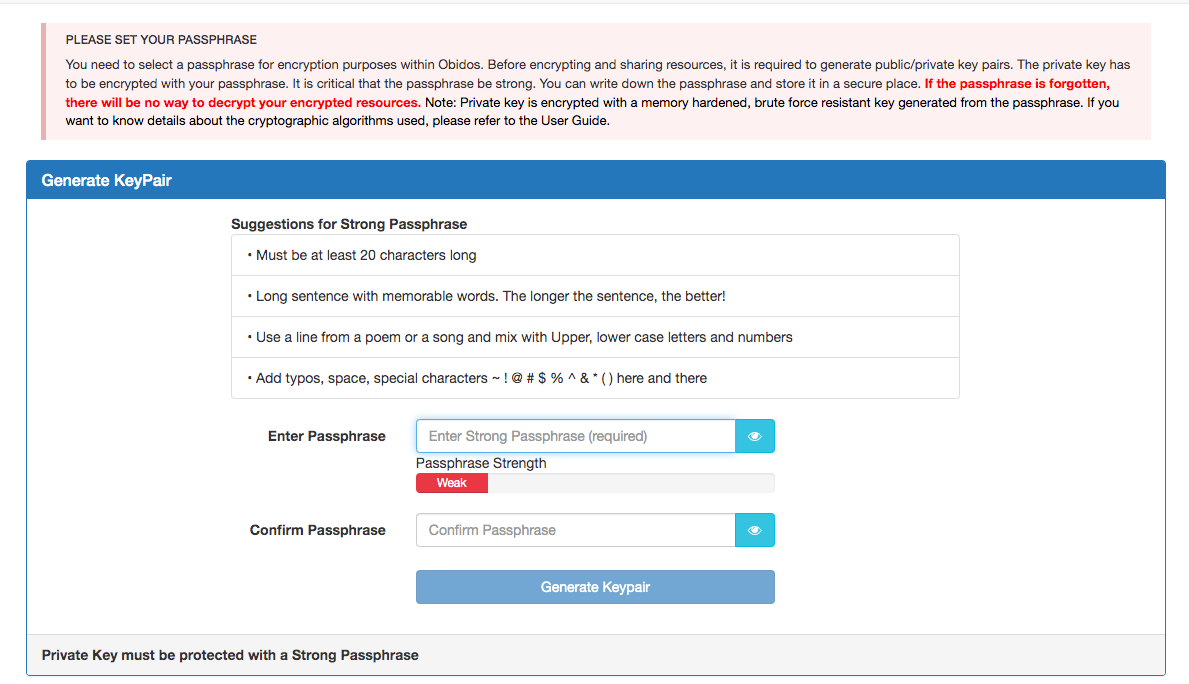
\includegraphics[width=90mm]{user/New-passphrase.png}
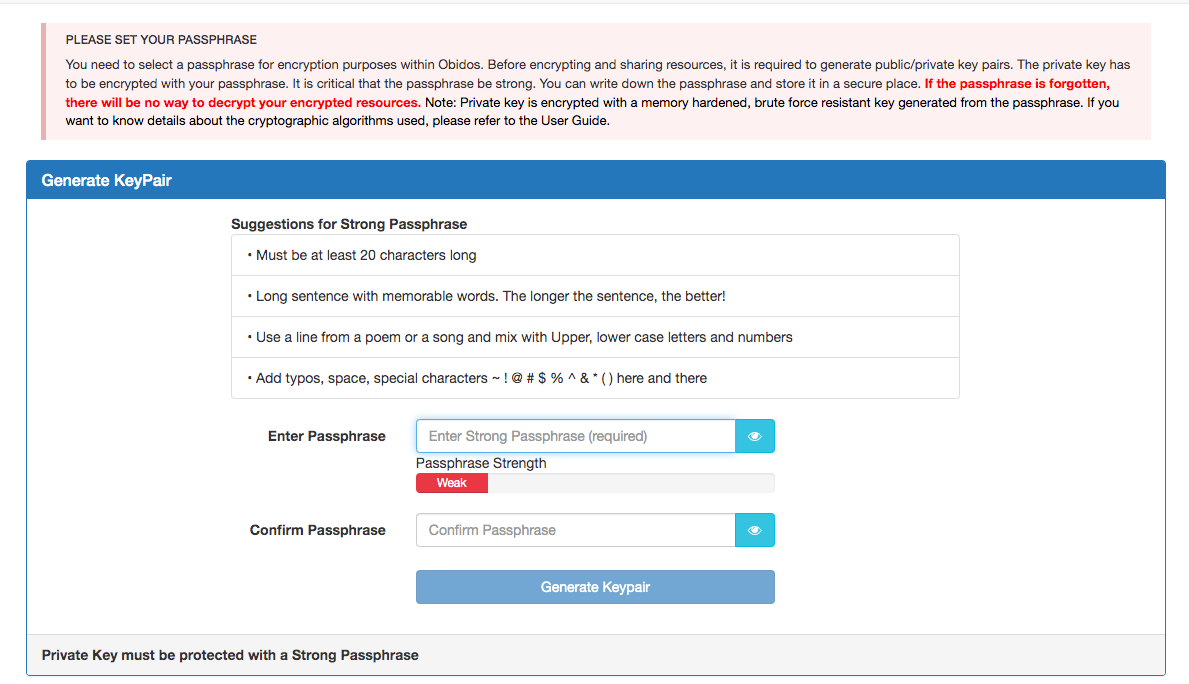
\includegraphics[scale=0.4]{user/New-passphrase.png}
\caption{Set New Passphrase}
\label{fig: Figure}
\end{figure}

A session is defined as the series of user interactions within Obidos once logged in till logout. 
The user can perform various activities during a session. 
Activities such as viewing an Item, sharing an Item, etc. requires the passphrase of the User. 
Instead of repeatedly entering the passphrase for each and every activity in the session, the User can provide the passphrase once for that session.
When a user logs into Obidos, there is an option to supply the passphrase for that session (see next Figure).
The session ends when the User logs out voluntarily or gets logged out by Obidos after a predefined period of inactivity.


\begin{figure}[H]
\centering
%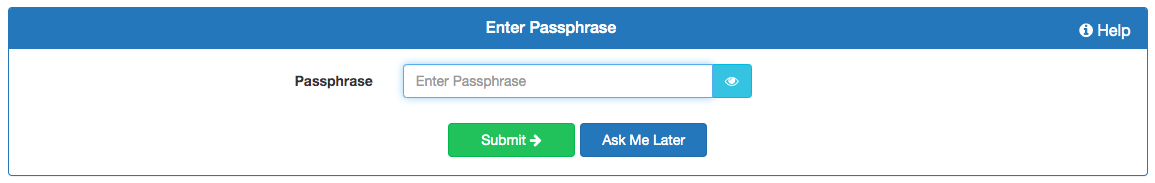
\includegraphics[width=90mm]{user/Login-Passphrase.png}
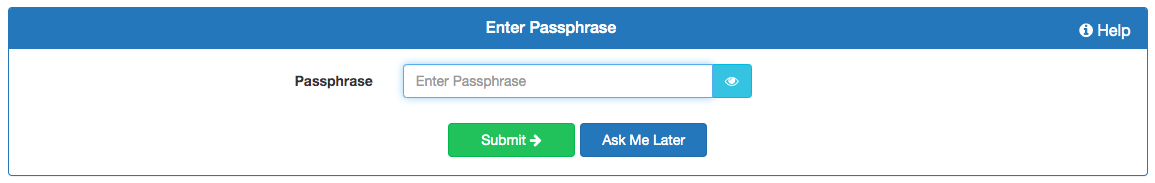
\includegraphics[scale=0.4]{user/Login-Passphrase.png}
\caption{Session Passphrase Activity}
\label{fig: Figure}
\end{figure}

If the passphrase is provided at the time of logging in, the User does not have to provide the passphrase
again for activities during that session.
If the passphrase is not provided at the time of logging in, the User can provide the passphrase at a later
point during the session.

Details of changing passphrase are given in the Chapter "Personal Preferences and Options".

\section{Logging Out}

The user can log out from a session using the Logout Menu Item from top right panel.

\begin{figure}[H]
\centering
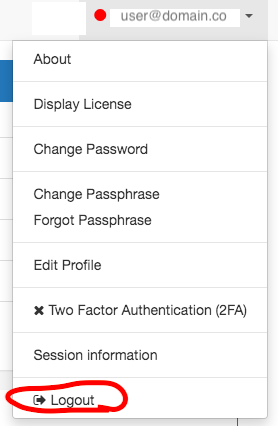
\includegraphics[scale=0.4]{user/Logout.png}
\caption{Logout menu}
\label{fig: Figure}
\end{figure}

In case there is no activity in the session for 30 minutes, the session will timeout and the User will be presented with a warning.

\begin{figure}[H]
\centering
%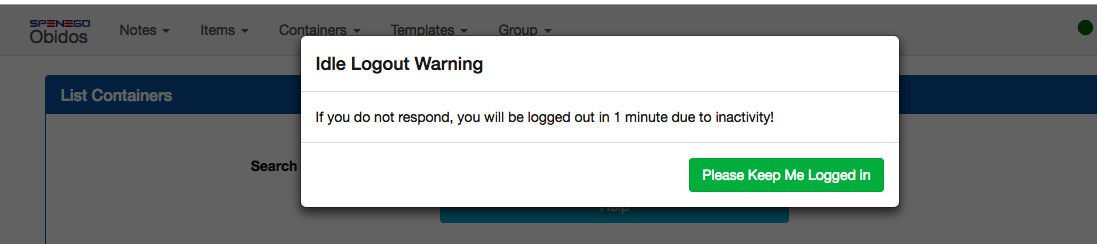
\includegraphics[width=90mm]{user/Inactivity.png}
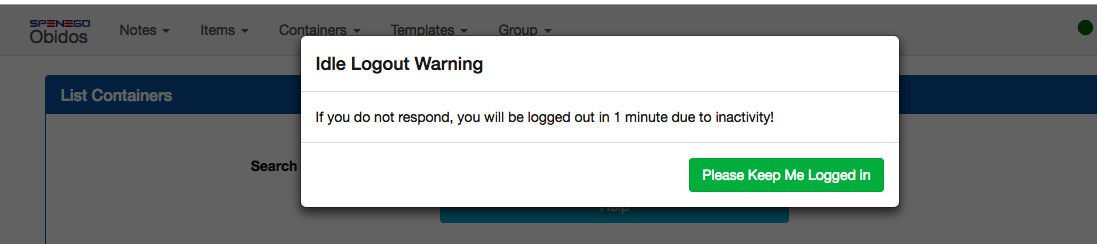
\includegraphics[scale=0.4]{user/Inactivity.png}
\caption{Inactivity Warning}
\label{fig: Figure}
\end{figure}

If the User fails to respond, the system will log out the User.

